% Slide 2: instance -> CNN -> partition of unity -> Whitney lift -> reduced solve -> certificate -> accept or fall back.
\documentclass[border=8pt]{standalone}
% Shared preamble for the slide diagrams. Palette and ink colours match figures/make_figures.py.
\usepackage[T1]{fontenc}
\usepackage{dejavu}
\renewcommand{\familydefault}{\sfdefault}
\usepackage{amsmath,amssymb}
\usepackage{xcolor}
\usepackage{tikz}
\usetikzlibrary{arrows.meta,positioning,shapes.geometric,calc,fit,backgrounds,decorations.pathmorphing,patterns}

\definecolor{surface}{HTML}{FCFCFB}
\definecolor{ink}{HTML}{0B0B0B}
\definecolor{inktwo}{HTML}{52514E}
\definecolor{muted}{HTML}{898781}
\definecolor{gridc}{HTML}{E1E0D9}
\definecolor{axisc}{HTML}{C3C2B7}
\definecolor{cblue}{HTML}{2A78D6}
\definecolor{corange}{HTML}{EB6834}
\definecolor{cgreen}{HTML}{1BAF7A}
\definecolor{camber}{HTML}{EDA100}

\newcommand{\tg}[1]{{\scriptsize\color{inktwo}#1}}  % small secondary line inside a node

\pagecolor{surface}
\color{ink}

\tikzset{
  every node/.style={text=ink},
  % one box style; the argument is the role colour (blue learned, inktwo exact/fixed, corange verification, ...)
  box/.style={draw=#1, fill=#1!10, rounded corners=3pt, line width=0.9pt, align=center,
              inner xsep=6pt, inner ysep=5pt, minimum height=1.25cm, text width=2.75cm, font=\footnotesize},
  tag/.style={font=\scriptsize, text=inktwo, align=center},
  arr/.style={-{Stealth[length=5.5pt,width=4.5pt]}, line width=0.9pt, color=inktwo},
  darr/.style={arr, dashed},
}

\begin{document}
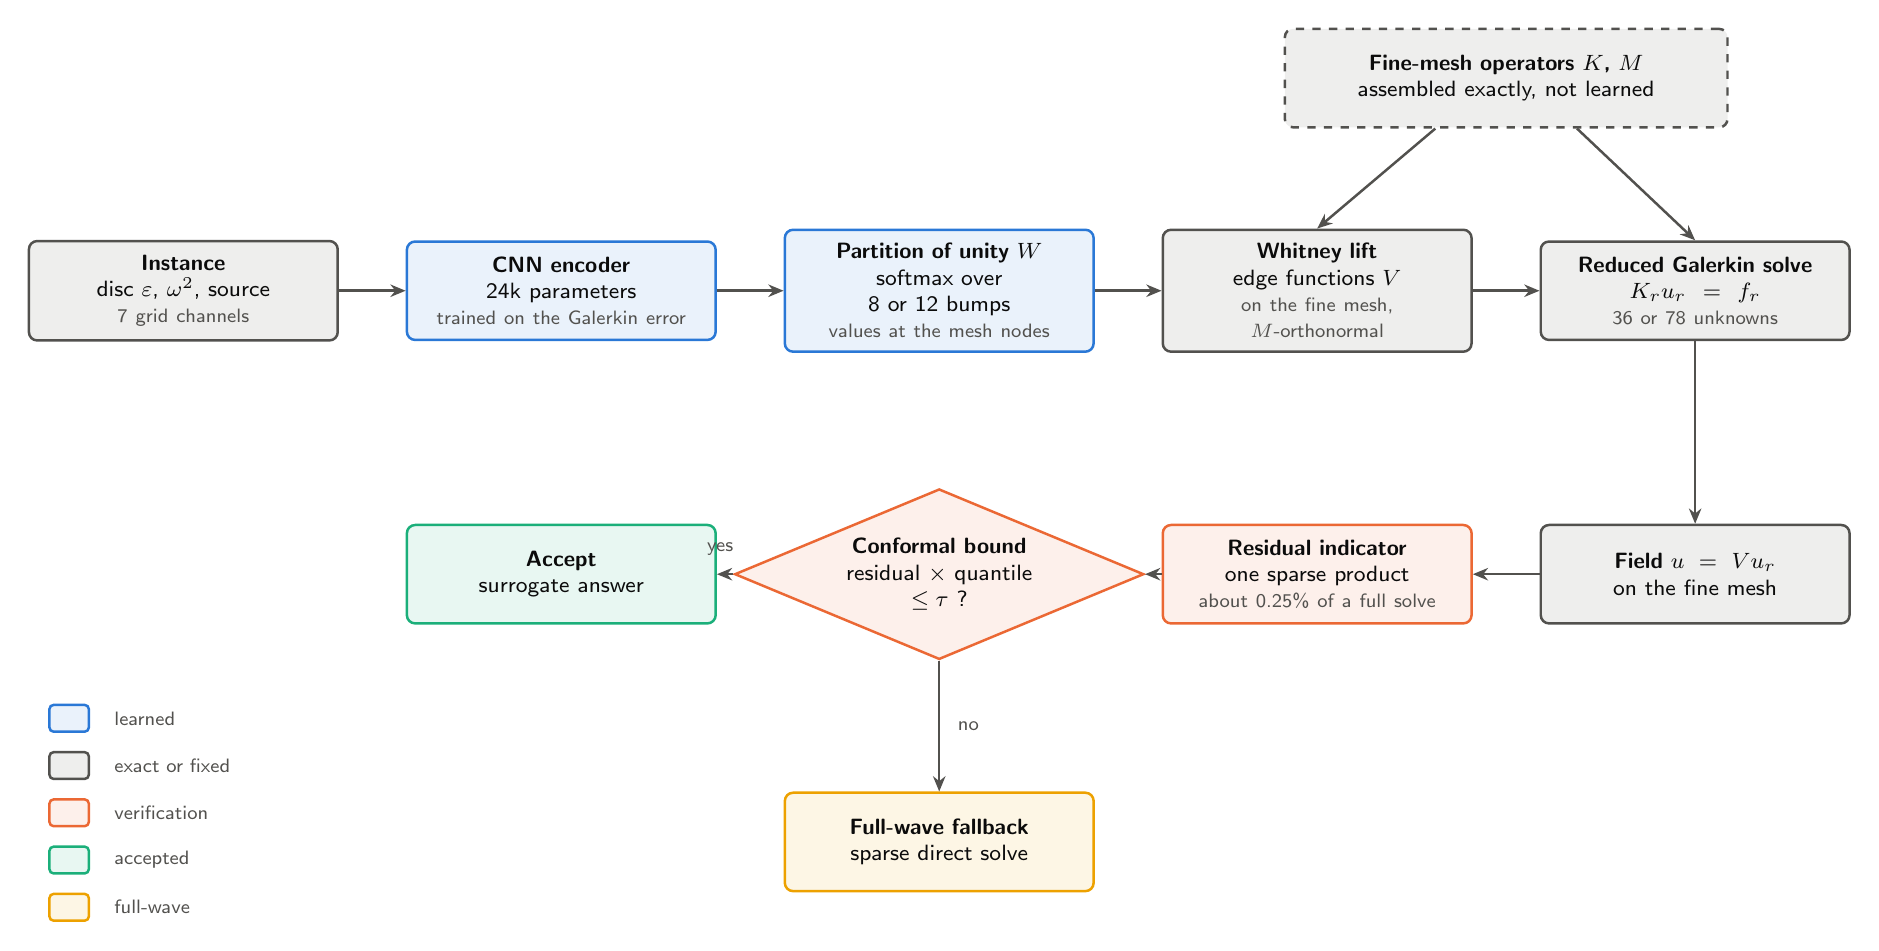
\begin{tikzpicture}[x=1cm,y=1cm, box/.append style={text width=3.5cm}]
  % ---- row 1: the learned basis and the reduced solve ----
  \node[box=inktwo]  (inst) at (0,0)    {\textbf{Instance}\\disc $\varepsilon$, $\omega^2$, source\\\tg{7 grid channels}};
  \node[box=cblue]   (cnn)  at (4.8,0)  {\textbf{CNN encoder}\\24k parameters\\\tg{trained on the Galerkin error}};
  \node[box=cblue]   (pou)  at (9.6,0)  {\textbf{Partition of unity $W$}\\softmax over 8 or 12 bumps\\\tg{values at the mesh nodes}};
  \node[box=inktwo]  (lift) at (14.4,0) {\textbf{Whitney lift}\\edge functions $V$\\\tg{on the fine mesh, $M$-orthonormal}};
  \node[box=inktwo]  (red)  at (19.2,0) {\textbf{Reduced Galerkin solve}\\$K_r u_r=f_r$\\\tg{36 or 78 unknowns}};

  \draw[arr] (inst) -- (cnn);
  \draw[arr] (cnn) -- (pou);
  \draw[arr] (pou) -- (lift);
  \draw[arr] (lift) -- (red);

  % exact fine-mesh operators
  \node[box=inktwo, dashed, text width=5.2cm] (ops) at (16.8,2.7)
        {\textbf{Fine-mesh operators $K$, $M$}\\assembled exactly, not learned};
  \draw[arr] ([xshift=-0.9cm]ops.south) -- (lift.north);
  \draw[arr] ([xshift=0.9cm]ops.south)  -- (red.north);

  % ---- row 2: lift back and check ----
  \node[box=inktwo]  (field) at (19.2,-3.6) {\textbf{Field $u=Vu_r$}\\on the fine mesh};
  \node[box=corange] (res)   at (14.4,-3.6) {\textbf{Residual indicator}\\one sparse product\\\tg{about 0.25\% of a full solve}};
  \node[draw=corange, fill=corange!10, line width=0.9pt, diamond, aspect=2.4, inner xsep=2pt, inner ysep=3pt,
        align=center, font=\footnotesize] (dec) at (9.6,-3.6) {\textbf{Conformal bound}\\residual $\times$ quantile\\$\le\tau$ ?};

  \draw[arr] (red)   -- (field);
  \draw[arr] (field) -- (res);
  \draw[arr] (res)   -- (dec);

  \node[box=cgreen] (acc)  at (4.8,-3.6)  {\textbf{Accept}\\surrogate answer};
  \node[box=camber] (fall) at (9.6,-7.0)  {\textbf{Full-wave fallback}\\sparse direct solve};
  \draw[arr] (dec) -- node[tag,above=3pt,pos=0.8]{yes} (acc);
  \draw[arr] (dec) -- node[tag,right=3pt]{no} (fall);

  % ---- legend ----
  \begin{scope}[shift={(-1.7,-5.6)}]
    \foreach \c/\t [count=\i from 0] in {cblue/learned, inktwo/exact or fixed, corange/verification, cgreen/accepted, camber/full-wave}{
      \draw[\c, fill=\c!10, line width=0.9pt, rounded corners=1.5pt] (0,-\i*0.6) rectangle +(0.5,0.34);
      \node[tag, anchor=west] at (0.7,-\i*0.6+0.17) {\t};
    }
  \end{scope}
\end{tikzpicture}
\end{document}
